\section{Theory}

\subsection{Cryogenics}
cryogenics roughly translates to ``the production of icy cold'' or the
``branch of physics which deals with the production of very low
temperatures and their effect on matter’’ -- Oxford English
Dictionary, 2nd edition, Oxford University Press (1989).
It is informally considered anything below around 170K.%%cite!!!!

\subsection{Cryogenic Cooling}
\begin{figure}[htbp]
\centering
\includegraphics{pics/pvdiagramhe4.pdf}
\caption{P-V diagram for helium-4. \label{fig:pvdiagramhe4}}
\end{figure}
Starting with a liquid helium sample in a cryostat it is possible to cool to lower temperatures by exploiting the phase transition lines as shows in a diagram in Figure \ref{fig:pvdiagramhe4}.
The sample \he\ is liquid in contact with vapour \he. As the sample is equilibrium
it must lie on the phase transition line of liquid to vapour. By attaching a vacuum pump and
slowly pumping on the vapour the pressure is reduced, as the pressure goes down the sample is still in equilibrium on the phase line, so the boiling point, and temperature, of the sample goes down, on Figure \ref{fig:pvdiagramhe4}
this is a down and to the left direction.
The vapour pressures and corresponding temperatures of the \he\ have been measured
so that in the following experiment low temperature thermometry not a complication
and the pressure measurements can be converted into temperatures.

The theoretical limit of cooling it at $T=0$K, although imposable to reach.
There is still energy in the system, called zero-point energy.
\he\ is special because even at $0$K the Van Der Walls forces (Figure \label{fig:vanderwallsforces}) between the atoms
are too strong to cause \he\ to become solid.


\begin{figure}[htbp]
\centering
\includegraphics{pics/vanderwallsforces.pdf}
\caption{Van Der Walls forces acting as springs between atoms \label{fig:vanderwallsforces}}
\end{figure}


\subsection{Superfluids}
%for a superfluid to exist there needs to be a condensate, a 
\begin{figure}[htb]
\centering
\includegraphics{pics/groundstateoccupation.pdf}
\caption{Qualitative graph showing how the distribution $N$ of atoms depending on energy $E$, $N(E)$
changes between two example temperatures above a transition point, here labeled $T_B$.
The large peak at low $E$ is intended to show ground state occupation. \label{fig:groundstateoccupation}}
\end{figure}
Helium 4 is a ``composite boson'' with net spin of zero, made of just two protons, two neutrons, and two electrons. As a boson it mostly follows Bose-Einstein statistics and at low temperatures Bose-Einstein condensation describes the formation of superfluid as atoms `condense’ to the ground energy state and become indistinguishable.
The mass condensation of atoms to the ground state leads to a macroscopic occupation of the ground state.

The transition to ground state begins at a lambda point.
Below the lambda point helium (\he) becomes superfluid. Called \he II above the lambda point 
and below called \he I, for first (I) and second (II) state of liquid \he.

An property of \he-II is the apparent loss of all viscosity, figure \ref{fig:superfluid}.

\begin{figure}[htb]
\centering
\includegraphics[width = 0.6\textwidth]{pics/superfluid.JPG}
\caption{Photograph of superfluid in a demonstration cryostat (clear glass) having just passed 
through a superleak, a fluid with only zero viscosity can do.\label{fig:superfluid}}
\end{figure}

At the transition point the heat capacity of the system dramatically increases, Figure \ref{fig:cvtdiagram}.
The peak of the heat capacity is rounded by other fields adding potentials across the fluid.

In the laboratory, it is the height of the superfluid and the 
gravitational potential energy across the
container that add a small variation of the
ground state energy\footnote{In space, where the potential from gravity changes less across the
container, the Cv peak is much higher, as tested on the ISS}.
Because of the 
This `rounding' of the ground state is enough to make the transition surmountable\cite{microgravity}.

\begin{figure}[htb]
\centering
\includegraphics{pics/cvtdiagram.pdf}
\caption{$C_v$ - T diagram showing heat capacity peaking over the transition temperature. \label{fig:cvtdiagram}}
\end{figure}

\subsection{Cryostat Design}
\begin{figure*}[htbp]
\centering
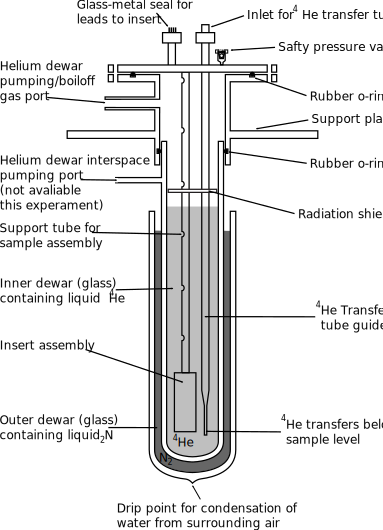
\includegraphics{pics/dewar.pdf}
\caption{Example of dewar used in the lab. Image based on Shaun Fisher's PHYS352 course material \cite{dewarimage}.
Main alterations are style, formatting, layout, and the addition of the safety valve for the inner dewar. \label{fig:dewar}}
\end{figure*}
Cryostats are designed to reduce the heat flow $\dot{Q}$ from the laboratory environment, at $\approx 300$K,
to the cryogenic liquid, $\approx 2\to4$K. 

Dewars themselves are good insulators from conduction as the vacuum between the 
glass layers actually gets better under lower temperature, the renaming gas
in the vacuum  will `stick' (energetically beneficial) to
the colder surface and no longer shuttle heat between the two vacuum surfaces.

To reduce the black body radiation heating up the Helium
the outer surface of the dewars are coated in a shiny metallic foil.

\begin{equation}
\dot{Q}_\text{blackbody} = \sigma \epsilon A T^4 \label{equ:bb1}
\end{equation}
$\sigma$ is the Stephan Boltzmann constant at $5.68 \times 10^{-8}$,
and $\epsilon$ is the emissivity of the surface, a value that changes between
$0$ for a none emitting surface, and $1$ for a perfect black body.
By reducing the emissivity, $\epsilon$, of the glass by coating it in silver,
the total amount of heat $\dot{Q}$ it absorbs from radiation.

Equation \ref{equ:bb1} is only for the black body radiation in one direction,
Black body radiation is a a two way process, absorption of heat $\dot{Q}_\text{in}$
from black body radiation and the emission of heat $\dot{Q}_\text{out}$
with the same process. So the total heat absorbed is Equation \ref{equ:bb2}.

\begin{equation}
\dot{Q}_\text{total} = \sigma \epsilon A \left( T_{\text{hot}}^4 - T_\text{cold}^4 \right) \label{equ:bb2}
\end{equation}

With $T_{\text{hot}} \approx 300$K and $T_{\text{cold}} \approx 4$K, the total heat $\dot{Q}$ is
still very high for practical purposes, so a intermediary layer of liquid Nitrogen is added so that for the
inner dewar only $T_{\text{hot}} \approx 77$K (boiling point of Nitrogen)

Baffles or Radiation shields inside the inner dewar reduce radiation down into 
the liquid. The baffles are cooled by the vapour evaporating off the Helium and
so do not just re-emit radiation down.

Another major heat source for the liquid Helium is the support tube, Equation \ref{equ:cond}. So it
is constructed out of a thin tube to reduce the cross-sectional area and
made from Stainless steel for the low thermal conductivity.
\begin{equation}
\dot{Q}_\text{conduction} = \frac{A}{L} \bar{k} \Delta T \label{equ:cond}
\end{equation}
$\bar{k}$ is the average conductivity over the range $\Delta T$.

An example cryostat implementing both a Nitrogen layer and baffles is shown in Figure \ref{fig:dewar}.

\subsection{Two fluid model}
The two fluid model is a phenomenological macroscopic \emph{model} used to
explain the characteristics of superfluids, although there is no microscopic theory supporting this.%CITE
The fluid is treated as two totally inter-penetrating non-interacting fluids.
The two distinct fluids are called the components of the fluid.
There is no actual physics separation in the normal and super components.
The density of the normalfluid and superfluid are related with Equation \ref{equ:densitysuperfulid}
\begin{equation}
\rho = \rho_n + \rho_s \label{equ:densitysuperfulid}
\end{equation}
The subscripts $s$ as the superfluid components and $n$ for the normal component.
The superfluid is identified with the ground state energy level Bose-Einstein
condensate and the normal fluid with the excitation above that ground state.

The superfluid component has a velocity $\vec{v}_s$, zero viscosity,
zero entropy ($\to$ zero temperature (third law)), and irrotational flow ($\nabla \times \vec{v}_s$).

While the normal component still behaves classically as a fluid with
velocity $\vec{v}_n$ with viscosity and entropy carrying temperature.
The proportion of superfluid and normalfluid components change over
temperature as more atoms are in the ground state.
Figure \label{fig:normalsuperfraction} shows qualitatively the
change in proportion of the two components.
Above the transition temperature (here $T_\lambda$) of superfluidity 
only the normal component exists so $\rho_n / \rho = 1$.
At idealistic $T=0$, only the superfluid component exists, $\rho_s / \rho = 1$.

%%pic of superfluid normal fluid components changing over temperature
\begin{figure}[htb]
\centering
\includegraphics{pics/normalsuperfraction.pdf}
\caption{Superfluid and normal fluid components changing over temperature.\label{fig:normalsuperfraction}}
\end{figure}

The \he II becomes `pure’ at temperatures under about .5k, but the pumping cooling method
as a practical limit of about 1K as there are no longer enough atoms evaporating off the
gas to reduce the temperature over losses by heat in.

\subsection{Counterflow}
With a heat source inside a superfluid normalfluid mix,
heat converts superfluid to normalfluid, and the normalfluid carries entropy
away from the heat source while the rest of the fluid acts as a heatsink.
The normalfluid reverts to superfluid at the heatsink.
This means that superfluid flows towards the heat source and normalfluid flows away from the heat source.
The superfluid is a superconductor of heat and has huge thermal conductivity. 
There can be no steady state thermal gradients in the superfluid, because of the efficient transition of the heat.

\subsection{Thermohydrodynamical Equations}
With the hydrodynamical system and the hydrodynamical system that is a superfluid
there are 6 Thermohydrodynamical Equations:

\begin{itemize}
\item Total fluid density \begin{equation}\rho = \rho_n + \rho_s\end{equation}
\item Momentum current density \begin{equation}\vec{j} = \rho_n\vec{v}_n + \rho_s\vec{v}_s\end{equation}
\item Entropy conservation \begin{equation}\nabla \cdot \left( \rho S \vec{v}_n \right) = - \frac{\partial \left( \rho S \right)}{ \partial t}\end{equation}
\item Acceleration equation \begin{equation}\frac{\partial \vec{v}_s}{\partial t} = S \nabla T - \frac{1}{\rho} \nabla P\end{equation}
\item Mass continuity \begin{equation}\nabla \cdot \vec{j} = - \frac{\partial \rho}{\partial t}\end{equation}
\item Euler’s equation (negating viscosity) \begin{equation} \frac{\partial \vec{j}}{\partial t} = - \nabla P\end{equation}
\end{itemize}

Hydrodynamical equations for normalfluid have density $\rho$ and pressure $P$
as variables which can be arranged to pressure-density waves. This is just sound,
or first sound.
But with the thermohydrodynamical equations another pair of variables, entropy $S$ and
temperature $T$ can result in a entropy-temperature wave equation, this is the second sound.
\begin{equation}
\frac{\partial^2 S }{ \partial t^2} = \underbrace{-\frac{\rho_s}{\rho_n}S^2}_\text{velocity} \nabla^2 T 
\end{equation}
In this entropy-temperature wave, $S$ and $T$ oscillate in phase. 
%%show steps from 6equations to wave equation...

For second sound waves the velocity squared ($c^2$) is related to to coefficient
in front of the spacial derivative of the variable $T$, so:
\begin{equation}
c^2 = \frac{\rho_s}{\rho_n} S^2 \left( \frac{\partial T}{\partial S} \right)_{p} 
\end{equation}
as $ C_v = T\left(\frac{\partial S}{\partial T} \right)_{\rho, V} $ then
\begin{equation}
c^2 = \frac{\rho_s}{\rho_n}\frac{TS^2}{C_v} \label{equ:c2rsrnts2cv}
\end{equation}
The second sound wave will have alternating regions of high $T$ to low $T$
while high $S$ to low $S$ and normal component density high $\rho_n$ to low $\rho_n$
then in antiphase low $\rho_s$ to high $\rho_s$ etc.
As with the counterflow earlier the $\vec{v}_n$
flows away from $T$ and $\vec{v}_s$ flows towards $T$.
These changes are drawn in Figure \ref{fig:normalossilations}.

%Inside a region of second sound the overall momentym is constant
%$ \rho_n\vec{v}_n + \rho_s\vec{v}_s = 0 $

%%picture of superfluid ossilations in superfluid fraction.

In addition to second sound there are third and forth sounds are from applying
different boundary conditions the six thermohydrodynamical equations.
Third sound is in the thin superfluid films and fourth sound are in superleaks
where the normal fluid is clamped because of the viscosity to the porous superleak.

\subsection{Second sound}
In the propagation of entropy and heat as a wave
the temperature is held in the normalfluid component of the superfluid, as $S=0$
for the superfluid component, see also Figure \ref{fig:normalossilations}.
The waves can can be generated by adding cyclic variations of heat,
this transmits very well in the normal component and is propagated
because of the counterflow and very good thermal conductivity of the superfluid
component.

\begin{figure}[htbp]
\centering
\includegraphics{pics/normalossilations.pdf}
\caption{Oscillating components of superfluid and normal fluid.\label{fig:normalossilations}}
\end{figure}

Resonances of second sound will start with high entropy at the
heat source and will `bounce' of the resonance chamber opposite wall at a 
high region of entropy, unlike compared to  first sound in 
a closed pipe with pressure fixed.


% put in theory:nitorgen pumping?
%%asside, how the nitrogen is pumped out of the dewer
\subsection{Cryogenic Fluid Pumping \label{sec:cryopumping}}
With nitrogen, the liquid in the transfer dewar is pumped
out by opening a heat exchanger valve on the
top of the dewar, this boils some of the nitrogen back into the 
dewar.
As the boiled nitrogen is less dense the top space above the
liquid is pressurised. The liquid nitrogen is forced out of a
transfer tube positioned at the bottom, well below the level of the liquid.

With helium there is no need for a heat exchanger pipe on the transfer dewar as
the removable transfer tube is enough to get pressure to pump helium.
Additional complication arise from helium, but these are to conserve wastage.










